\documentclass[12pt]{article}
\usepackage[margin=1in]{geometry}
\usepackage[table]{xcolor}
\usepackage{graphicx}
\usepackage{booktabs}
\usepackage{float}
\usepackage{amsmath}
\usepackage{hyperref}
\usepackage{fancyhdr}
\usepackage{caption}
\usepackage{pdflscape}
\usepackage{tikz} % Added TikZ package
\usepackage{xcolor} % Required for defining custom colors
\usetikzlibrary{positioning, arrows.meta, shapes.geometric} % Added TikZ libraries


% Set header and footer
\pagestyle{fancy}
\fancyhf{}
\fancyhead[L]{USC Facilities: Rain Barrel Water Pump System}
\fancyfoot[C]{\thepage}

\begin{document}

\title{
    \vspace{2in}
    \textbf{EMCH427-002} \\[1ex]
    \textbf{Preliminary Design Review} \\[1ex]
    \textbf{Sponsor: USC Facilities} \\[1ex]
    \vspace{2in}
}

\author{
    \textbf{Team Members:} \\[2ex]
    Tanner Harmon\\[1ex]
    Presston McConnell\\[1ex]
    William Wenzel\\[1ex]
    Jacob Vaught\\[2ex]
}

\date{}

\maketitle
\thispagestyle{fancy}

\newpage

\section{Project Background}

\begin{itemize}
    \item \textbf{Sponsor:} Office of Sustainability in Green Quad
    \item \textbf{Project Context:} Currently, rainwater collected in barrels is not being utilized effectively. This project aims to use the collected rainwater to irrigate surrounding plants, enhancing water conservation and reducing manual irrigation efforts.
    \item \textbf{Stakeholders:} Office of Sustainability, garden volunteers, nearby residents, and garden walkers.
\end{itemize}

\section{Needs}
\subsection{Comprehensive Needs} 
Refer to Tables 1a to 1g in the Appendix for the complete list of needs.

\subsection{Critical to Quality Needs} 
\begin{table}[H]
\centering
\caption*{Table 3: Ranking of Critical to Quality (CTQ) needs.}
\rowcolors{2}{lightgray}{}
\begin{tabular}{|p{10cm}|c|c|c|c|c|}
\hline
\textbf{Need} & \textbf{\#1} & \textbf{\#2} & \textbf{\#3} & \textbf{\#4} & \textbf{Sum} \\
\hline
1.1. The system should minimize the time required to transfer water from the tank to the garden. & 6 & 6 & 6 & 6 & 24 \\
\hline
1.3. Water distribution should cover the entire garden area efficiently. & 3 & 4 & 2 & 5 & 14 \\
\hline
2.1. The system should provide sufficient pressure for effective water delivery. & 4 & 5 & 5 & 3 & 17 \\
\hline
2.10. The system should provide adequate flow rate for all intended watering methods. & 5 & 3 & 4 & 4 & 16 \\
\hline
5.10. The system should be designed to minimize noise pollution. & 2 & 2 & 3 & 2 & 9 \\
\hline
7.1. The system should comply with all relevant safety standards. & 1 & 1 & 1 & 1 & 4 \\
\hline
\end{tabular}
\end{table}

\subsection{Mission Statement} 
USC Facilities needs a water distribution system that ensures fast transfer, sufficient pressure, adequate flow, complete garden coverage, and compliance with safety standards.


\section{Engineering Characteristics}

\subsection{Critical Engineering Characteristics}

\begin{itemize}
    \item \textbf{Water Transfer Rate (gal/min)}\\
    \textbf{Target:} 12--16 gal/min \\
    \textbf{Fallback:} 8--12 gal/min \\
    \textbf{Importance:} Ensures efficient irrigation, reducing time and labor required for watering sessions, directly impacting operational efficiency and water conservation goals.

    \item \textbf{Water Pressure (psi)}\\
    \textbf{Target:} 40--60 psi \\
    \textbf{Fallback:} 20--40 psi \\
    \textbf{Importance:} Guarantees effective water distribution across the garden, preventing issues like uneven watering and ensuring reliable sprinkler operation.

    \item \textbf{Energy Consumption (kWh/year)}\\
    \textbf{Target:} $\leq\$50$ per year \\
    \textbf{Fallback:} $\leq\$150$ per year \\
    \textbf{Importance:} Minimizes operational costs and supports sustainability objectives by reducing the system's carbon footprint and energy usage.

    \item \textbf{Potable Water Savings (gallons/month)}\\
    \textbf{Target:} $\geq$800 gallons/month \\
    \textbf{Fallback:} $\geq$500 gallons/month \\
    \textbf{Importance:} Maximizes water conservation by reducing the reliance on potable water sources, aligning with USC's sustainability initiatives.

    \item \textbf{Noise Level (dB)}\\
    \textbf{Target:} $\leq$40 dB at 5 yards \\
    \textbf{Fallback:} $\leq$50 dB at 5 yards \\
    \textbf{Importance:} Maintains a quiet operational environment, preventing noise pollution and ensuring user comfort on campus.
\end{itemize}

\newpage
\section{Selected Concept Details}

\subsection{System Description}

Key components of the Rain Barrel Pressurizer include:

\begin{itemize}
    \item \textbf{Solar Power System:} Solar panels + 100Ah battery
    \item \textbf{120V AC Pump:} 1525 GPH, 115VAC, $\tfrac{3}{4}$ hp Pump + 1500W Inverter
    \item \textbf{Dual Spigots:} Two spigots, allowing for pressurized or manual operation.
    \item \textbf{Pump House:} A pump cover made from reclaimed material that protects the pump.
    \item \textbf{Winterization Features:} Designed to allow pipes to be drained for winterization.
\end{itemize}


\begin{figure}[H]
    \centering
    
\includegraphics[width=\textwidth]{PDR/System.png} % Replace with actual image file
    \caption{System-Level view}
    \label{fig:clustering}
\end{figure}

\subsection{System Issues}

\begin{itemize}
    \item \textbf{Poor Spigot Placement for Draining:} Spigot is not optimally located for drainage.
    \item \textbf{Thermally Inadequate Cover Material:} Current material is not inuslative enough.
    \item \textbf{Low Battery Capacity:} The battery may not sustain long usage, reducing reliability.
    \item \textbf{Poor Solar Panel Placement:} Solar panel placement reduces sunlight and energy.
\end{itemize}

\subsection{Strengths of the System}

\begin{itemize}
    \item \textbf{Manual and Automatic Water Usage Methods:} Offers operation flexibility.
    \item \textbf{Simple, Integrated System:} Ensures ease of use and maintenance.
\end{itemize}

\subsection{Plans to Minimize Failures}

\begin{itemize}
    \item \textbf{Battery Capacity Evaluation:} Energy consumption analysis to determine if a larger battery is necessary.
    \item \textbf{Optimize Solar Panel Placement:} Inspect site to identify the best location(s) for solar panels.
    \item \textbf{Winterization Protocols:} Develop user manual with winterization directions.
\end{itemize}

\begin{figure}[H]
    \centering
    
\includegraphics[width=\textwidth]{PDR/Top-Down.png} % Replace with actual image file
    \caption{Top Down View}
    \label{fig:clustering}
\end{figure}
\subsection{Prototype Feasibility}

Building a physical prototype for the Rain Barrel Water Pump System is deemed infeasible due to budgetary and time constraints. Instead, the focus \textit{should} shift to final product development, using simulations and engineering analyses to validate design choices and address identified challenges.


% ------------------------------------------------------------
% Section: Schematic Layout of Total Concept
% ------------------------------------------------------------
\section{Schematic Layout of Total Concept}
\label{sec:schematic_layout}

\subsection{Illustration of Clustering}
\label{subsec:clustering_illustration}

\begin{figure}[H]
    \centering
    
\includegraphics[width=\textwidth]{Product_Architecture/component_layout.png} % Replace with actual image file
    \caption{Subsystem Clustering of the Rain Barrel Water Pump System}
    \label{fig:clustering}
\end{figure}

\subsubsection{Rationale of Clustering}
The clustering of components into subsystems was guided by the following principles:
\begin{itemize}
    \item \textbf{Functionality Grouping:} Components are put together to streamline maintenance. 
    \item \textbf{Modularity:} Subsystems operate independently to allow repairs.
    \item \textbf{Interaction Minimization:} Clustering reduces incidental interactions, such as heat or vibration transfer, between unrelated components.
\end{itemize}

\subsubsection{Unintended/Consequential Interactions:}
\begin{itemize}
    \item \textbf{Heat Build-Up:} The pump/battery/inverter/charge controller generates heat.
    \item \textbf{Vibrations:} Pump operation causes vibrations that may loosen connections.
    \item \textbf{Corrosion:} Water leakage risks corrosion of electrical components.
\end{itemize}

\subsubsection{Plans to minimize interactions:}
\begin{itemize}
    \item Heat management via spacing and heat-resistant materials.
    \item Vibration damping pads and flexible fittings.
    \item Corrosion prevention with weatherproof enclosures and proper sealing.
\end{itemize}

\subsection{Geometric Layout of Design}
\label{subsec:geometric_layout}

The geometric layout shows the system's size and arrangement. A layout is in Figure \ref{fig:geometric_layout_2d}.

\begin{figure}[H]
    \centering
    
\includegraphics[width=\textwidth]{Product_Architecture/geometric_layout.png} % Replace with actual 2D image file
    \caption{2D Geometric Layout of the Rain Barrel Water Pump System}
    \label{fig:geometric_layout_2d}
\end{figure}

\subsubsection{Dimensions}
\begin{itemize}
    \item \textbf{Pump House:} 2 ft (L) $\times$ 4 ft (W) $\times$ 3 ft (H)
    \item \textbf{Rain Tank:} 5 ft (L) $\times$ 5 ft (W) $\times$ 7 ft (H)
    \item \textbf{Solar Panel:} 2 ft (L) $\times$ 3 ft (W) $\times$ 3 ft (H)
    \item \textbf{Battery:} 1 ft (L) $\times$ 1 ft (W) $\times$ 1 ft (H)
\end{itemize}

\subsubsection{Rationale for Arrangement and Sizing}
\begin{itemize}
    \item \textbf{Space Efficiency:} Components are arranged compactly to minimize the system's footprint while maintaining accessibility.
    \item \textbf{Maintenance Access:} Frequently serviced components, such as the pump and battery, are placed at the front for easy access.
    \item \textbf{Interaction Minimization:} Adequate spacing prevents incidental heat and vibration interactions.
\end{itemize}




\subsection{Additional Illustrations}

\begin{figure}[H]
    \centering
    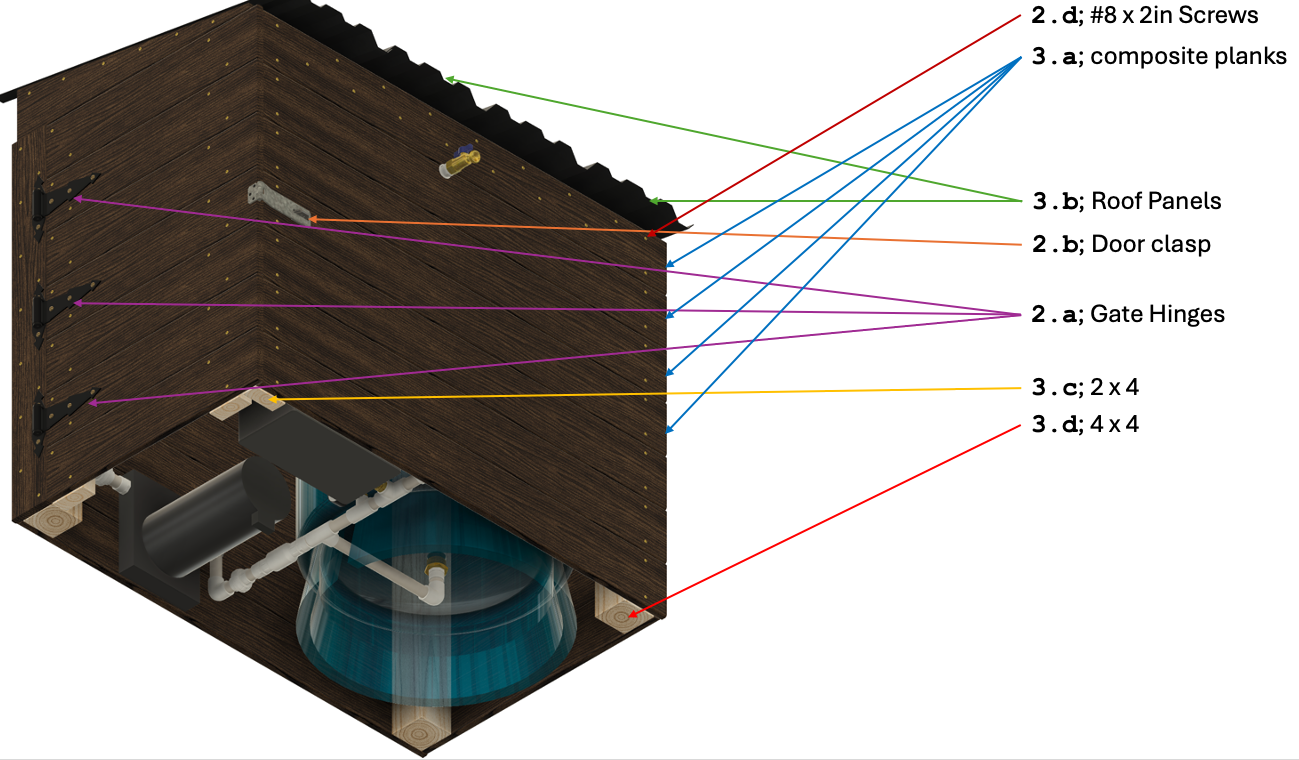
\includegraphics[width=0.8\textwidth]{Housing_View.png}
    \caption{Housing View of the Pump System}
    \label{fig:housingview}
\end{figure}

\begin{figure}[H]
    \centering
    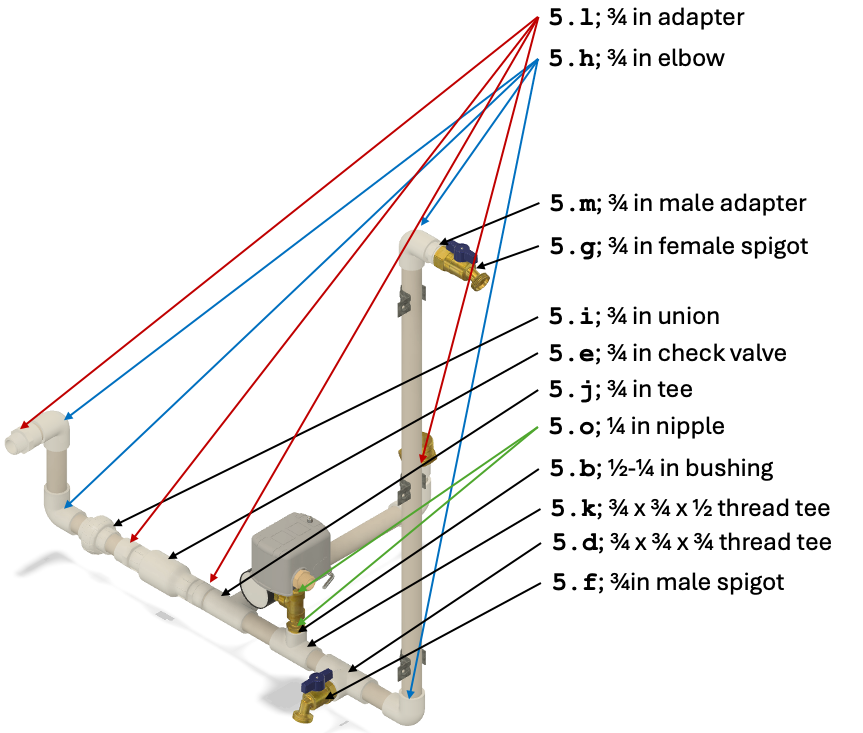
\includegraphics[width=0.7\textwidth]{Internal_Pipe.png}
    \caption{Internal Pipe Configuration}
    \label{fig:internalpipe}
\end{figure}

\begin{figure}[H]
    \centering
    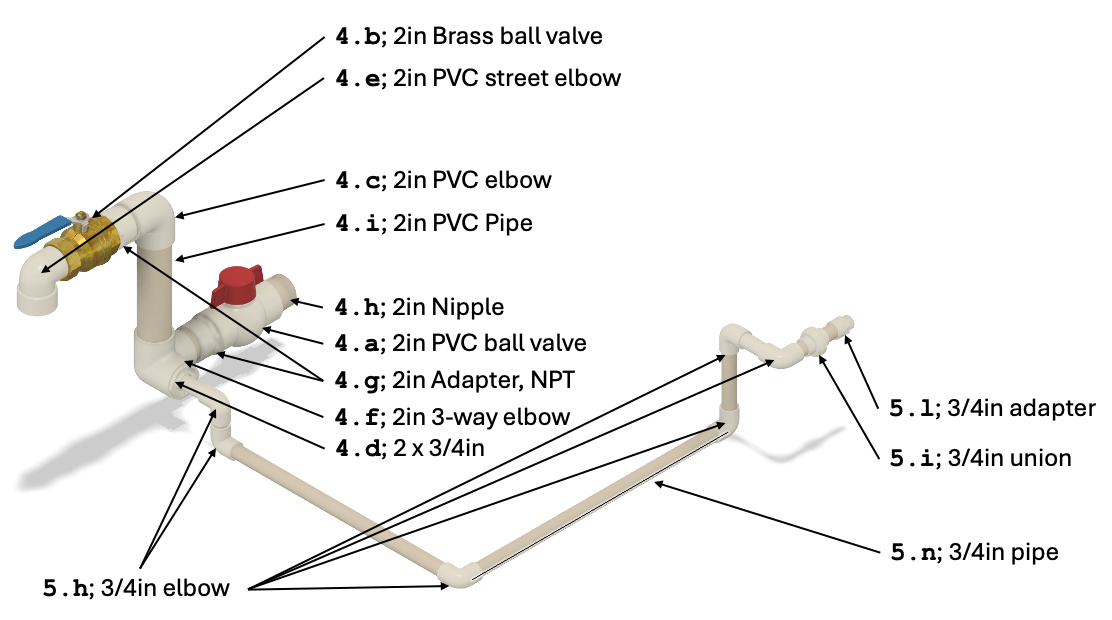
\includegraphics[width=\textwidth]{External_Pipe.png}
    \caption{External Pipe Layout}
    \label{fig:externalpipe}
\end{figure}

\begin{figure}[H]
    \centering
    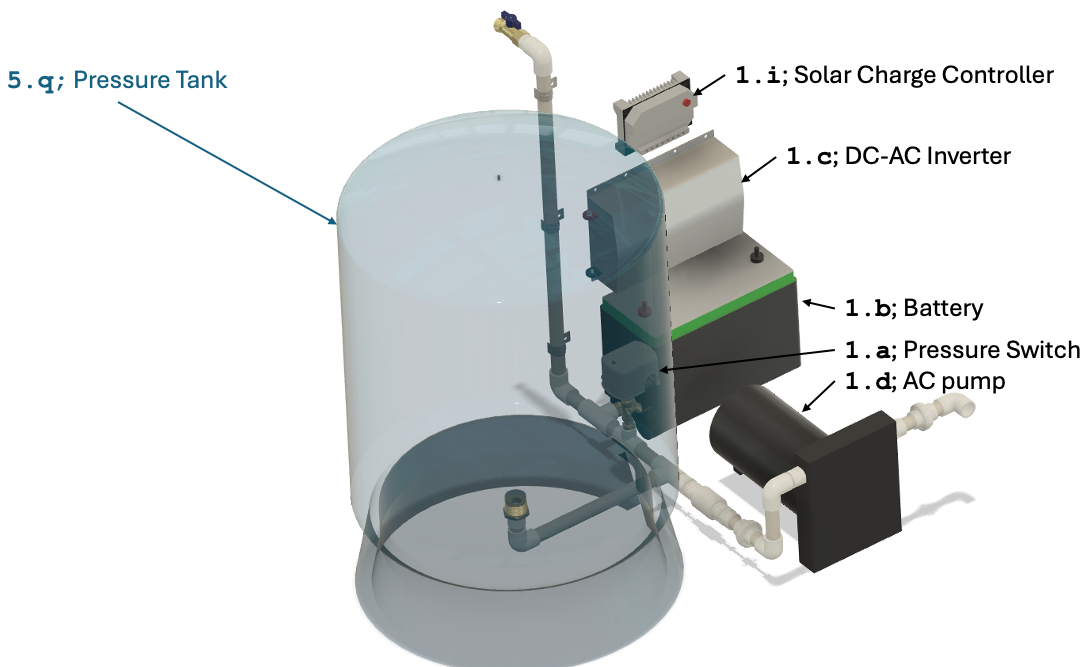
\includegraphics[width=\textwidth]{Pump_House.png}
    \caption{Pump House Design}
    \label{fig:pumphouse}
\end{figure}


\section{Identification of TBDs}
\label{sec:tdbs}

\subsection{Solar Panel Placement}
\label{subsec:solar_panel_placement}

\textbf{Issue:} Optimal placement of solar panels is undecided due to building and trees. Mounting on the building may be required.
\newline
\textbf{Actions to Resolve:}
\begin{itemize}
    \item Conduct a site survey to identify mounting locations.
    \item Assess impact of obstructions on efficiency.
    \item Explore mounting options.
\end{itemize}
\newline
\textbf{Timeline:} Decision expected by mid-December.

\subsection{Battery Expansion and Capacity}
\label{subsec:battery_expansion}

\textbf{Issue:} Battery may not be enough to run Inverter and pump. Space is already set aside for additional batteries.
\newline
\textbf{Actions to Resolve:}
\begin{itemize}
    \item Perform energy analysis for adding batteries.
    \item Assess if existing solar panels support expanded capacity.
\end{itemize}
\newline
\textbf{Timeline:} Evaluation to be completed by end of December.

\subsection{Timeline Overview}
\label{subsec:timeline_overview}


\begin{table}[H]
    \centering
    \caption{Timeline for TBD Resolutions}
    \label{tab:tdb_timeline}
    \begin{tabular}{|p{4cm}|p{6cm}|p{4cm}|}
    \hline
    \textbf{TBD} & \textbf{Actions to Resolve} & \textbf{Expected Completion} \\
    \hline
    Solar Panel Placement & Conduct site survey, assess obstructions, explore mounting options & Mid-December \\
    \hline
    Battery Expansion and Capacity & Perform cost analysis, assess solar capacity, explore battery technologies & End of December \\
    \hline
    System Winterization Features & Analyze weather data, select materials, integrate protective measures & Early January \\
    \hline
    \end{tabular}
\end{table}

% ------------------------------------------------------------
% Section: Preliminary Budget
% ------------------------------------------------------------
\section{Preliminary Budget}
\label{sec:preliminary_budget}

\subsection{Material Costs}

The total estimated material cost for the project is \$1,170.53. Including a 25\% contingency fee for shipping, handling, and taxes brings the total to \$1,463.16.

\subsubsection{High-Cost Items}

The following items are identified as high-cost components within the budget:

\begin{itemize}
    \item \textbf{Inverter}
    \item \textbf{Pressure Tank}
    \item \textbf{Solar Panel}
    \item \textbf{Battery}
    \item \textbf{Charge Controller}
    \item \textbf{Low Water Detector}
\end{itemize}

\subsubsection{Detailed Material Budgets}

\begin{figure}[H]
    \centering
    \includegraphics[width=\textwidth]{table1.png}
    \caption{Table 1: Voltage System Budget}
    \label{fig:table1}
\end{figure}

\begin{figure}[H]
    \centering
    \includegraphics[width=\textwidth]{table2.png}
    \caption{Table 2: Housing System Budget}
    \label{fig:table2}
\end{figure}

\begin{figure}[H]
    \centering
    \includegraphics[width=\textwidth]{table3a.png}
    \caption{Table 3a: Watering System Budget}
    \label{fig:table3a}
\end{figure}

\begin{figure}[H]
    \centering
    \includegraphics[width=\textwidth]{table3b.png}
    \caption{Table 3b: Watering System Budget (Continued)}
    \label{fig:table3b}
\end{figure}

\subsubsection{Final Recommended Budget}
\begin{figure}[H]
    \centering
    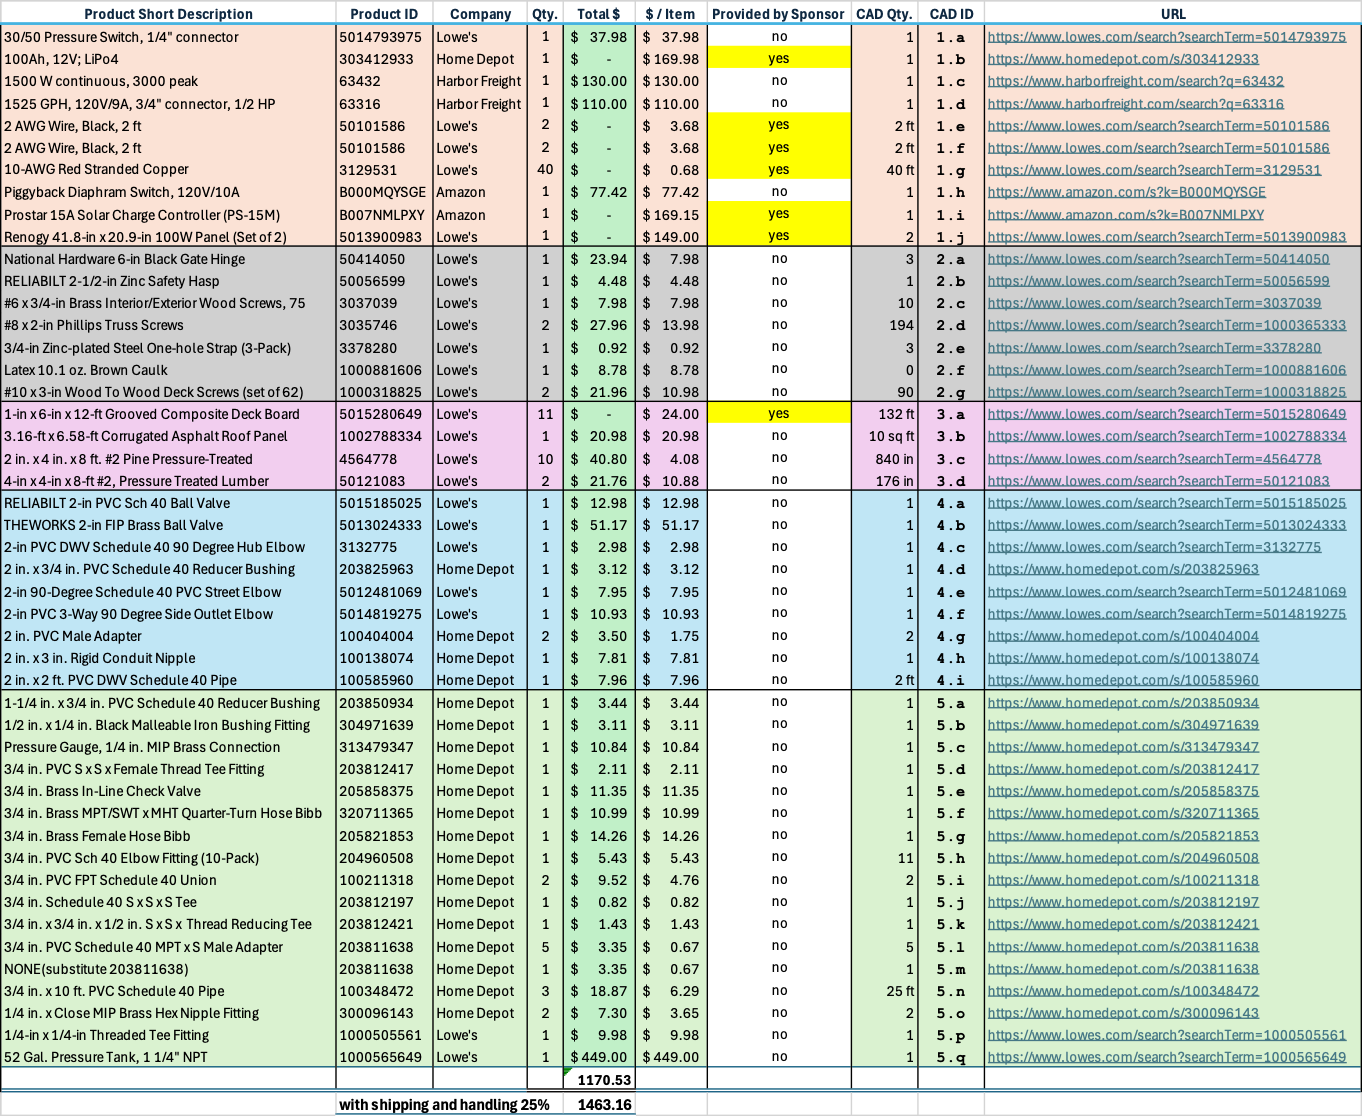
\includegraphics[width=0.9\textwidth]{budget.png}
    \caption{Final Budget Summary}
    \label{fig:final_budget}
\end{figure}

\subsection{Timeline for Ordering Materials and Resolving TBDs}
\begin{itemize}
    \item \textbf{Early December:}
    \begin{itemize}
        \item Finalize decisions on TBDs, particularly solar placement and battery expansion.
        \item Place orders for high-cost items to account for potential shipping delays.
    \end{itemize}
\end{itemize}
\section{Future Work}
\label{sec:future_work}

Moving forward, the project timeline is as follows:
\begin{itemize}
    \item \textbf{Dec--Feb:} Prototype construction.
    \item \textbf{Jan--Feb:} Detailed engineering analysis and modeling.
    \item \textbf{March:} Testing and refinement.
    \item \textbf{End of April:} Project completion.
\end{itemize}

\newpage



\newpage
% Change margins for one page
\newgeometry{margin=0.7in} % New margins

\section{Appendix}

\begin{table}[H]
\centering
\caption*{Table 1a: Operational efficiency needs.}
\label{table:1a}
\rowcolors{2}{lightgray}{}
\begin{tabular}{|p{10cm}|c|c|c|c|c|}
\hline
\textbf{Need} & \textbf{\#1} & \textbf{\#2} & \textbf{\#3} & \textbf{\#4} & \textbf{Sum} \\
\hline
1.1. The system should minimize the time required to transfer water from the tank to the garden. & 5 & 6 & 7 & 4 & \cellcolor{yellow}22 \\
1.2. The system must operate effectively with minimal manual intervention. & 0 & 1 & 0 & 0 & 1 \\
1.3. Water distribution should cover the entire garden area efficiently. & 4 & 4 & 2 & 5 & \cellcolor{yellow}15 \\
1.4. The system should be able to operate without frequent start-stop interruptions. & 0 & 0 & 0 & 1 & 1 \\
1.5. The system should ensure minimal water wastage during operation. & 3 & 1 & 0 & 2 & 6 \\
1.6. Water output should be consistent and reliable during the watering process. & 3 & 3 & 2 & 3 & \cellcolor{yellow}11 \\
1.7. The system should be flexible enough to handle varying watering schedules. & 0 & 0 & 4 & 1 & 5 \\
1.8. The system should be scalable to handle garden expansion or additional tanks. & 0 & 1 & 2 & 2 & 5 \\
1.9. The system should allow for easy monitoring of water usage and distribution. & 0 & 0 & 0 & 1 & 1 \\
1.10. The system should be able to adapt to water demand and supply conditions. & 0 & 0 & 0 & 0 & 0 \\
1.11. The system should maintain functionality during peak water demand periods. & 2 & 1 & 2 & 1 & 6 \\
1.12. The system should be easy to activate and deactivate when needed. & 3 & 2 & 5 & 2 & \cellcolor{yellow}12 \\
1.13. The system should be adaptable to changes in garden layout or design. & 0 & 0 & 0 & 0 & 0 \\
1.14. The system should be able to handle variable water volumes effectively. & 1 & 1 & 0 & 2 & 4 \\
1.15. The system should minimize the physical effort required to operate it. & 3 & 2 & 2 & 1 & \cellcolor{yellow}8 \\
1.16. The system should be easy to set up and configure for different garden zones. & 0 & 0 & 0 & 1 & 1 \\
1.17. The system should have the capability to adjust flow according to plant needs. & 0 & 0 & 0 & 0 & 0 \\
1.18. The system should be capable of rapid deployment or removal as needed. & 0 & 0 & 0 & 0 & 0 \\
1.19. The system should facilitate quick troubleshooting during operational issues. & 3 & 1 & 5 & 2 & \cellcolor{yellow}11 \\
1.20. The system should be able to resume operations seamlessly. & 2 & 1 & 1 & 1 & 5 \\
\hline
\end{tabular}
\end{table}

\restoregeometry % Revert to original margins

\newpage
\begin{table}[H]
\centering
\caption*{Table 1b: Pressure and flow needs.}
\label{table:1b}
\rowcolors{2}{lightgray}{}
\begin{tabular}{|p{10cm}|c|c|c|c|c|}
\hline
\textbf{Need} & \textbf{\#1} & \textbf{\#2} & \textbf{\#3} & \textbf{\#4} & \textbf{Sum} \\
\hline
2.1. The system should provide sufficient pressure for effective water delivery. & 3 & 2 & 5 & 2 & \cellcolor{yellow}12 \\
2.2. The system should maintain consistent pressure regardless of elevation. & 2 & 1 & 0 & 1 & 4 \\
2.3. The system should prevent significant pressure drops during operation. & 1 & 0 & 0 & 0 & 1 \\
2.4. The system should allow adjustment of pressure for different applications. & 0 & 0 & 0 & 0 & 0 \\
2.5. The system should provide feedback on water pressure for user awareness. & 0 & 0 & 0 & 0 & 0 \\
2.6. The system should be capable of maintaining pressure over long distances. & 2 & 2 & 0 & 3 & 7 \\
2.7. The system should ensure even water distribution across all garden areas. & 0 & 0 & 2 & 1 & 3 \\
2.8. The system should avoid pressure surges that could damage components. & 1 & 1 & 3 & 1 & 6 \\
2.9. The system should function effectively under varying pressure conditions. & 1 & 1 & 0 & 0 & 2 \\
2.10. The system should provide adequate flow rate for all intended watering methods. & 3 & 3 & 2 & 0 & \cellcolor{yellow}8 \\
2.11. The system should allow easy detection and correction of flow issues. & 0 & 0 & 0 & 0 & 0 \\
2.12. The system should be capable of maintaining flow in low-pressure scenarios. & 0 & 1 & 6 & 0 & 7 \\
2.13. The system should operate efficiently with varying water levels in the tank. & 4 & 4 & 2 & 3 & \cellcolor{yellow}13 \\
2.14. Water should reach all parts of the garden without pressure loss. & 3 & 3 & 0 & 2 & \cellcolor{yellow}8 \\
2.15. The system should support gradual changes in pressure to avoid spikes. & 1 & 1 & 0 & 0 & 2 \\
2.16. The system should allow for easy verification of flow performance. & 0 & 0 & 0 & 0 & 0 \\
2.17. The system should ensure minimal disruption to flow during adjustments. & 0 & 0 & 0 & 0 & 0 \\
2.18. The system should be able to function at both high and low flow rates. & 0 & 0 & 0 & 0 & 0 \\
2.19. The system should facilitate consistent flow under fluctuating conditions. & 1 & 2 & 0 & 2 & 5 \\
2.20. The system should maintain optimal flow for the intended irrigation method. & 3 & 3 & 0 & 0 & 6 \\
\hline
\end{tabular}
\end{table}

\newpage
\begin{table}[H]
\centering
\caption*{Table 1c: Usability needs.}
\label{table:1c}
\rowcolors{2}{lightgray}{}
\begin{tabular}{|p{10cm}|c|c|c|c|c|}
\hline
\textbf{Need} & \textbf{\#1} & \textbf{\#2} & \textbf{\#3} & \textbf{\#4} & \textbf{Sum} \\
\hline
3.1. The system should be easy for non-technical users to operate. & 4 & 3 & 6 & 4 & \cellcolor{yellow}17 \\
3.2. The system should provide clear instructions for use. & 3 & 2 & 1 & 3 & \cellcolor{yellow}9 \\
3.3. The system should be intuitive to set up and use with minimal training. & 2 & 2 & 2 & 1 & 7 \\
3.4. The system should be accessible to users with different physical capabilities. & 0 & 0 & 0 & 0 & 0 \\
3.5. The system should provide clear feedback on its operational status. & 0 & 0 & 0 & 0 & 0 \\
3.6. The system should be easy to start, stop, and adjust as needed. & 4 & 5 & 5 & 2 & \cellcolor{yellow}16 \\
3.7. The system should allow for quick learning and familiarization. & 2 & 2 & 2 & 1 & 7 \\
3.8. The system should be straightforward to configure for different watering needs. & 2 & 2 & 0 & 0 & 4 \\
3.9. The system should provide visible indicators of key operational parameters. & 0 & 0 & 0 & 0 & 0 \\
3.10. The system should minimize the number of steps required for operation. & 3 & 3 & 1 & 4 & \cellcolor{yellow}11 \\
3.11. The system should have easy-to-read and understand operational guidelines. & 1 & 1 & 0 & 1 & 3 \\
3.12. The system should be user-friendly in both daylight and low-light conditions. & 0 & 1 & 0 & 1 & 2 \\
3.13. The system should have clear labeling for all user-accessible components. & 1 & 0 & 0 & 0 & 1 \\
3.14. The system should allow for easy monitoring of its performance and settings. & 0 & 0 & 0 & 0 & 0 \\
3.15. The system should require minimal physical exertion to operate. & 2 & 1 & 0 & 1 & 4 \\
3.16. The system should be easy to reset or reconfigure if needed. & 0 & 0 & 1 & 0 & 1 \\
3.17. The system should facilitate quick and easy shutdown in case of emergency. & 0 & 1 & 0 & 1 & 2 \\
3.18. The system should be easy to use without the need for tools or equipment. & 2 & 1 & 1 & 3 & 7 \\
3.19. The system should allow users to operate it comfortably for extended periods. & 1 & 1 & 0 & 1 & 3 \\
3.20. The system should be designed to minimize errors during operation. & 2 & 2 & 4 & 2 & \cellcolor{yellow}10 \\
\hline
\end{tabular}
\end{table}

\newpage
\begin{table}[H]
\centering
\caption*{Table 1d: Maintenance needs.}
\label{table:1d}
\rowcolors{2}{lightgray}{}
\begin{tabular}{|p{10cm}|c|c|c|c|c|}
\hline
\textbf{Need} & \textbf{\#1} & \textbf{\#2} & \textbf{\#3} & \textbf{\#4} & \textbf{Sum} \\
\hline
4.1. The system should require minimal maintenance for reliable operation. & 4 & 5 & 3 & 2 & \cellcolor{yellow}14 \\
4.2. The system should allow easy access to components that need maintenance. & 0 & 1 & 0 & 1 & 2 \\
4.3. The system should have a low frequency of maintenance interventions. & 3 & 2 & 0 & 1 & 6 \\
4.4. The system should allow for identification of components that require servicing. & 0 & 0 & 0 & 1 & 1 \\
4.5. The system should be easy to clean and maintain regularly. & 2 & 1 & 0 & 1 & 4 \\
4.6. The system should provide indications when maintenance is needed. & 0 & 0 & 0 & 0 & 0 \\
4.7. The system should be designed to minimize the likelihood of component failure. & 1 & 2 & 2 & 2 & 7 \\
4.8. The system should be robust against wear and tear in normal conditions. & 3 & 2 & 3 & 1 & \cellcolor{yellow}9 \\
4.9. The system should allow for easy replacement of consumable parts. & 1 & 0 & 0 & 0 & 1 \\
4.10. The system should have a simple process for performing routine maintenance. & 0 & 0 & 0 & 1 & 1 \\
4.11. The system should be able to continue functioning with minor faults or wear. & 1 & 1 & 4 & 0 & 6 \\
4.12. The system should include features that prevent issues from escalating. & 0 & 0 & 0 & 0 & 0 \\
4.13. The system should be resistant to clogging and other common issues. & 1 & 2 & 0 & 0 & 3 \\
4.14. The system should minimize the need for specialized maintenance or skills. & 0 & 0 & 1 & 1 & 2 \\
4.15. The system should be durable under both indoor and outdoor conditions. & 0 & 0 & 0 & 0 & 0 \\
4.16. The system should have a clear and accessible maintenance log. & 0 & 0 & 0 & 1 & 1 \\
4.17. The system should allow for easy troubleshooting of common issues. & 0 & 1 & 0 & 1 & 2 \\
4.18. The system should be easy to drain and store if needed. & 0 & 0 & 0 & 0 & 0 \\
4.19. The system should have protection against damage from external elements. & 0 & 0 & 7 & 0 & 7 \\
4.20. The system should be easy to prepare for seasonal changes in weather. & 0 & 1 & 0 & 1 & 2 \\
\hline
\end{tabular}
\end{table}

\newpage
\begin{table}[H]
\centering
\caption*{Table 1e: Environmental impact needs.}
\label{table:1e}
\rowcolors{2}{lightgray}{}
\begin{tabular}{|p{10cm}|c|c|c|c|c|}
\hline
\textbf{Need} & \textbf{\#1} & \textbf{\#2} & \textbf{\#3} & \textbf{\#4} & \textbf{Sum} \\
\hline
5.1. The system should minimize its impact on the local environment. & 2 & 1 & 1 & 1 & 5 \\
5.2. The system should prioritize the use of sustainable and recyclable materials. & 1 & 1 & 2 & 1 & 5 \\
5.3. The system should be energy-efficient and use minimal power. & 2 & 2 & 0 & 2 & 6 \\
5.4. The system should not introduce contaminants to the water or soil. & 3 & 2 & 0 & 2 & 7 \\
5.5. The system should be designed to reduce water wastage. & 0 & 1 & 0 & 2 & 3 \\
5.6. The system should align with sustainability goals of the project site. & 2 & 2 & 2 & 0 & 6 \\
5.7. The system should not disrupt local wildlife or their habitats. & 0 & 0 & 0 & 1 & 1 \\
5.8. The system should be compatible with existing eco-friendly practices on-site. & 1 & 1 & 2 & 0 & 4 \\
5.9. The system should support the collection and use of renewable resources. & 0 & 1 & 1 & 1 & 3 \\
5.10. The system should be designed to minimize noise pollution. & 3 & 2 & 4 & 2 & \cellcolor{yellow}11 \\
5.11. The system should be easily integrated into the existing infrastructure. & 0 & 0 & 0 & 0 & 0 \\
5.12. The system should be resistant to environmental factors like extreme weather. & 0 & 1 & 0 & 0 & 1 \\
5.13. The system should be designed to minimize its carbon footprint. & 2 & 2 & 0 & 2 & 6 \\
5.14. The system should promote the conservation of natural resources. & 0 & 0 & 0 & 0 & 0 \\
5.15. The system should support practices that reduce soil erosion. & 0 & 0 & 0 & 0 & 0 \\
5.16. The system should be able to adapt to changing environmental regulations. & 0 & 0 & 0 & 0 & 0 \\
5.17. The system should not contribute to the pollution of local water sources. & 0 & 1 & 0 & 2 & 3 \\
5.18. The system should use materials that are safe for human interaction. & 1 & 2 & 3 & 2 & \cellcolor{yellow}8 \\
5.19. The system should be compatible with rainwater harvesting practices. & 3 & 4 & 0 & 1 & \cellcolor{yellow}8 \\
5.20. The system should last many years with minimal environmental impact. & 2 & 2 & 5 & 1 & \cellcolor{yellow}10 \\
\hline
\end{tabular}
\end{table}

\newpage
\begin{table}[H]
\centering
\caption*{Table 1f: Cost and budgetary needs.}
\label{table:1f}
\rowcolors{2}{lightgray}{}
\begin{tabular}{|p{10cm}|c|c|c|c|c|}
\hline
\textbf{Need} & \textbf{\#1} & \textbf{\#2} & \textbf{\#3} & \textbf{\#4} & \textbf{Sum} \\
\hline
6.1. The system should be cost-effective to implement within the given budget. & 2 & 1 & 4 & 1 & \cellcolor{yellow}8 \\
6.2. The system should have low operational costs once installed. & 1 & 1 & 0 & 1 & 3 \\
6.3. The system should not exceed the specified maximum budget. & 2 & 1 & 1 & 2 & 6 \\
6.4. The system should prioritize cost-saving without compromising performance. & 0 & 0 & 0 & 1 & 1 \\
6.5. The system should allow for flexible budgeting and cost adjustments. & 0 & 0 & 0 & 0 & 0 \\
6.6. The system should avoid ongoing costs that are disproportionately high. & 0 & 0 & 0 & 1 & 1 \\
6.7. The system should leverage available resources to minimize expenses. & 0 & 0 & 0 & 0 & 0 \\
6.8. The system should provide value for money in terms of durability and efficiency. & 1 & 1 & 2 & 1 & 5 \\
6.9. The system should minimize the need for expensive consumables or parts. & 1 & 1 & 2 & 1 & 5 \\
6.10. The system should have a predictable cost structure for maintenance. & 0 & 0 & 3 & 0 & 3 \\
6.11. The system should facilitate potential cost recovery through operation. & 0 & 0 & 0 & 0 & 0 \\
6.12. The system should include a breakdown of anticipated costs and benefits. & 0 & 1 & 0 & 1 & 2 \\
6.13. The system should allow for potential upgrades within the existing budget. & 0 & 0 & 0 & 0 & 0 \\
6.14. The system should be designed with cost-effectiveness in mind from the start. & 0 & 0 & 2 & 0 & 2 \\
6.15. The system should be easy to scale without significant cost increases. & 0 & 0 & 1 & 0 & 1 \\
6.16. The system should not incur unexpected costs during installation or operation. & 0 & 0 & 0 & 0 & 0 \\
6.17. The system should utilize durable components to reduce replacement costs. & 0 & 0 & 4 & 0 & 4 \\
6.18. The system should be designed to minimize financial risk to stakeholders. & 0 & 0 & 0 & 0 & 0 \\
6.19. The system should include provisions for cost-efficient disposal or recycling. & 0 & 0 & 0 & 0 & 0 \\
6.20. The system should consider long-term financial implications of its use. & 0 & 1 & 0 & 1 & 2 \\
\hline
\end{tabular}
\end{table}


\newpage
\begin{table}[H]
\centering
\caption*{Table 1g: Safety and compliance needs.}
\label{table:1g}
\rowcolors{2}{lightgray}{}
\begin{tabular}{|p{10cm}|c|c|c|c|c|}
\hline
\textbf{Need} & \textbf{\#1} & \textbf{\#2} & \textbf{\#3} & \textbf{\#4} & \textbf{Sum} \\
\hline
7.1. The system should comply with all safety standards. & 3 & 2 & 2 & 2 & \cellcolor{yellow}9 \\
7.2. The system should be safe to use in various weather. & 0 & 1 & 0 & 2 & 3 \\
7.3. The system should include measures to prevent accidental misuse. & 2 & 3 & 0 & 2 & 7 \\
7.4. The system should be free from sharp edges or hazardous components. & 1 & 1 & 2 & 1 & 5 \\
7.5. The system should not pose any risks to pedestrians or garden users. & 1 & 2 & 2 & 3 & \cellcolor{yellow}8 \\
7.6. The system should have clear labeling to indicate potential hazards. & 1 & 1 & 0 & 2 & 4 \\
7.7. The system should prevent water contamination that could pose health risks. & 0 & 0 & 0 & 0 & 0 \\
7.8. The system should be able to withstand accidental impacts without failure. & 0 & 0 & 0 & 1 & 1 \\
7.9. The system should not obstruct emergency access or exits. & 0 & 0 & 0 & 1 & 1 \\
7.10. The system should have measures to prevent unauthorized access. & 0 & 0 & 0 & 1 & 1 \\
7.11. The system should comply with local environmental regulations. & 0 & 0 & 0 & 1 & 1 \\
7.12. The system should not interfere with existing infrastructure or utilities. & 0 & 0 & 0 & 1 & 1 \\
7.13. The system should be designed to prevent tripping or slipping hazards. & 1 & 1 & 0 & 1 & 3 \\
7.14. The system should be stable and secure when in use and when not in use. & 2 & 1 & 0 & 1 & 4 \\
7.15. The system should not generate harmful emissions or pollutants. & 0 & 0 & 0 & 1 & 1 \\
7.16. The system should have clear instructions for safe operation. & 0 & 1 & 0 & 3 & 4 \\
7.17. The system should be designed to minimize the risk of fire or hazards. & 0 & 0 & 0 & 0 & 0 \\
7.18. The system should ensure that all components are properly secured. & 0 & 1 & 0 & 1 & 2 \\
7.19. The system should be resistant to vandalism or accidental damage. & 0 & 0 & 0 & 1 & 1 \\
7.20. The system should have emergency shut-off procedures clearly documented. & 1 & 1 & 0 & 2 & 4 \\
\hline
\end{tabular}
\end{table}

\end{document}
